\chapter{Statistik: Daten beschreiben und Schlüsse ziehen}

\section{Wozu Statistik?}

Statistik hilft uns, aus Daten sinnvolle Aussagen zu gewinnen, ohne uns von Einzelfällen, Ausreissern oder geschickt gestalteten Grafiken täuschen zu lassen.
In diesem Kapitel arbeiten wir mit kleinen, realistischen Datensätzen und üben das Zusammenspiel von
\begin{center}
	\textbf{Fragestellung \ $\rightarrow$\ Daten \ $\rightarrow$\ Beschreibung \ $\rightarrow$\ Schlussfolgerung}.
\end{center}

\begin{myattention}
	Statistik ist keine Rechenakrobatik, sondern schult das \textbf{rigorose Denken}:
	Welche Daten liegen vor? Was darf man damit berechnen? Und was bedeutet das Ergebnis in Worten?
\end{myattention}

\begin{myremark}
	Wir unterscheiden in diesem Kapitel bewusst zwei Perspektiven:
	\begin{itemize}
		\item \textbf{Beschreibende Statistik}: Daten einer Stichprobe ordnen, visualisieren und zusammenfassen.
		\item \textbf{Schliessende Statistik}: Von einer Stichprobe auf eine grössere Grundgesamtheit schliessen.
	\end{itemize}
\end{myremark}

\section{Was ist eine gute statistische Fragestellung?}

\begin{mydefinition}
	Eine \textbf{statistische Fragestellung} untersucht eine Grösse, die zwischen Personen, Gruppen oder Zeitpunkten \textbf{variiert}.
	Die Fragestellung soll so formuliert sein, dass Daten erhoben oder ausgewertet und danach begründet interpretiert werden können.
\end{mydefinition}

\begin{myexample}
	\textbf{Weniger geeignet}: ``Wer ist der Grösste in der Klasse?''

	\textbf{Statistisch geeignet}: ``Wie ist die Verteilung der Körpergrössen in der Klasse?''
\end{myexample}

\begin{myattention}
	Viele erste Ideen von Lernenden sind noch nicht statistisch formuliert. Häufig stehen einzelne Personen im Zentrum (``Wer ist die:der Schnellste?'')
	oder nur ein Thema ohne klare Messgrösse (``Ich möchte mehr über Familien wissen.'').
	Für Statistik braucht es stattdessen eine \textbf{Variable}, die bei mehreren Personen beobachtet wird.
\end{myattention}

\begin{myremark}
	Eine gute Fragestellung ist möglichst klar bezüglich Zielgruppe (für wen gilt die Aussage?),
	Variable (was genau wird gemessen?) und Vergleich (zwischen Gruppen, Zeitpunkten oder gegenüber einem Referenzwert).

	Typische, statistisch ergiebige Fragetypen sind:
	\begin{enumerate}
		\item \textbf{Verteilung einer Variable}: Wie viele? Wie häufig? Was ist typisch oder durchschnittlich?
		\item \textbf{Vergleich von Gruppen}: Gibt es Unterschiede oder Gemeinsamkeiten zwischen Gruppen?
		\item \textbf{Beziehung zwischen zwei Variablen}: Hängen zwei Merkmale zusammen?
		\item \textbf{Vorhersage auf Basis von Daten}: Lässt sich aus den Daten eine Tendenz oder Prognose ableiten?
	\end{enumerate}
\end{myremark}

\begin{mydefinition}
	\textbf{Repräsentativ} bedeutet: Die Stichprobe bildet die relevante Grundgesamtheit ausreichend gut ab.
	Wenn z.B. nur Lernende einer Schule im Alter 15--17 befragt werden, sind Aussagen für diese Gruppe möglich, aber nicht automatisch für alle Jugendlichen.
\end{mydefinition}

\begin{mydefinition}
	\textbf{Signifikant} bedeutet im statistischen Sinn: Ein beobachteter Unterschied oder Zusammenhang ist so deutlich, dass er nicht auf rein zufällige Variationen zurückzuführen ist.
	Signifikant ist nicht automatisch gleichbedeutend mit ``gross'', ``wichtig'' oder ``pädagogisch relevant''. Es geht hier um eine statistische Bewertung der Daten, nicht um eine inhaltliche Interpretation.
\end{mydefinition}

\begin{myexercise}
	Formulieren Sie die Fragestellung
	\begin{center}
		``Ist Schlafdauer mit Fokus verbunden?''
	\end{center}
	präziser für folgende Stichprobe: Lernende der Kantonsschule Lee, 15--17 Jahre.

	\begin{myanswer}
		Eine präzisere Formulierung wäre z.B.: ``Gibt es in unserer Stichprobe von Lee-Lernenden (15--17 Jahre) einen statistisch nachweisbaren sowie signifikanten Zusammenhang zwischen Schlafdauer und Fokus-Score?''

		Die Aussage gilt dann zunächst nur für diese Zielgruppe. Für breitere Aussagen müsste die Stichprobe erweitert werden.
	\end{myanswer}
\end{myexercise}

\begin{myexercise}[Fragestellung für Maturitätsarbeit]
	Untersuchen Sie Ihre eigene Maturitätsarbeitsidee und formulieren Sie eine präzise statistische Fragestellung, die sich mit den Daten, die Sie erheben oder analysieren möchten, beantworten lässt.
\end{myexercise}

\section{Daten und Skalenniveaus}

\subsection{Was sind Daten?}
Daten sind beobachtete oder erhobene Werte zu einer Fragestellung.
Oft stammen sie aus Umfragen, Messungen, Protokollen oder Apps (z.B.\ Schlaftracking).

\begin{mydefinition}\label{mydefinition:variable}
	Eine \textbf{Variable} ist eine Eigenschaft, die bei verschiedenen Personen oder Objekten unterschiedliche Werte annehmen kann.
\end{mydefinition}

\begin{myexample}
	Die Variable \textit{Schlafdauer} kann für verschiedene Personen unterschiedliche Werte (z.B.\ $6.5$ Stunden, $7.2$ Stunden, \dots) annehmen.
\end{myexample}

\subsection{Skalenniveaus (Skalenwerte)}
Das \textbf{Skalenniveau} (auch: Messniveau) bestimmt, welche Aussagen und Rechnungen sinnvoll sind.

\begin{mydefinition}\label{mydefinition:skalenniveau}
	Ein \textbf{Skalenniveau} beschreibt, welche Struktur eine Variable besitzt (nur Kategorien? Rangordnung? Abstände? echter Nullpunkt?)
	und legt damit fest, welche Kennzahlen und Diagramme sinnvoll sind.
\end{mydefinition}

\begin{myremark}
	Wenn das Skalenniveau unklar ist, helfen zwei Fragen:
	\begin{itemize}
		\item Gibt es eine \textbf{Reihenfolge} (mehr/weniger)?
		\item Sind \textbf{Abstände} oder sogar \textbf{Verhältnisse} (doppelt so viel) sinnvoll?
	\end{itemize}
\end{myremark}

\begin{mydefinition}\label{mydefinition:nominalskala}
	\textbf{Nominalskala:} Kategorien ohne Ordnung.

	\textbf{Beispiele}: Lieblingsfach, Wohnort, Musikgenre.
\end{mydefinition}

\begin{mydefinition}\label{mydefinition:ordinalskala}
	\textbf{Ordinalskala:} Kategorien mit Rangordnung, aber die Abstände zwischen Werten sind nicht sinnvoll interpretierbar.

	\textbf{Beispiele}: Zufriedenheit (1--5), Schulnoten, Ranglisten.
\end{mydefinition}

\begin{mydefinition}\label{mydefinition:intervallskala}
	\textbf{Intervallskala:} Gleiche Abstände sind sinnvoll, aber es gibt keinen echten Nullpunkt. Daher sind Verhältnisaussagen (z.B.\ doppelt so viel) nicht sinnvoll.

	\textbf{Beispiel}: Temperatur in \textdegree C (0\textdegree C bedeutet nicht ``keine Temperatur''). Vergleiche wie etwa 20\textdegree C ist doppelt so warm wie 10\textdegree C sind nicht sinnvoll, da der Nullpunkt willkürlich ist.
\end{mydefinition}

\begin{mydefinition}\label{mydefinition:verhältnisskala}
	\textbf{Verhältnisskala (Ratioskala):} Gleiche Abstände \textbf{und} echter Nullpunkt. Verhältnisaussagen sind sinnvoll.

	\textbf{Beispiele}: Länge, Gewicht, Zeitdauer, Temperatur in Kelvin. Bei der Temperatur in Kelvin ist 0 K der absolute Nullpunkt, was bedeutet, dass es keine negative Temperatur gibt und Verhältnisaussagen wie ``20 K ist doppelt so warm wie 10 K'' sinnvoll sind. Ähnliches gilt auch für Länge, Gewicht und Zeitdauer, da sie ebenfalls einen echten Nullpunkt haben (0 cm bedeutet keine Länge, 0 kg bedeutet kein Gewicht, 0 Sekunden bedeutet keine Zeitdauer).
\end{mydefinition}

\subsection{Übersicht der Skalenniveaus}

\begin{table}[H]
	\centering
	\small
	\begin{tabular}{l c c c c c}
		\toprule
		\textbf{Skalenniveau} & \textbf{Ordnung} & \textbf{Abstände} & \textbf{Nullpunkt} & \textbf{Lagemasse} & \textbf{Streuungsmasse}       \\
		\midrule
		Nominal               & \xmark           & \xmark            & \xmark             & Modus              & ---                           \\
		Ordinal               & \cmark           & \xmark            & \xmark             & Median, Modus      & \acrshort{IQR}                \\
		Intervall             & \cmark           & \cmark            & \xmark             & Mittelwert, Median & \acrshort{SD}, \acrshort{IQR} \\
		Verhältnis            & \cmark           & \cmark            & \cmark             & Mittelwert, Median & \acrshort{SD}, \acrshort{IQR} \\
		\bottomrule
	\end{tabular}
	\caption{Übersicht der Skalenniveaus und geeignete statistische Kennzahlen}
	\label{table:skalenniveaus}
\end{table}

\begin{myremark}
	Je höher das Skalenniveau, desto mehr Rechenoperationen und statistische Verfahren sind möglich.
	Bei Unsicherheit: Lieber ein niedrigeres Niveau wählen (konservativer Ansatz).
\end{myremark}

\begin{myexercise}\label{myexercise:skalenniveaus-zuordnen}
	Ordnen Sie den folgenden Variablen ein Skalenniveau zu (Nominal / Ordinal / Intervall / Verhältnis):
	\begin{itemize}
		\item Schlafdauer in Stunden
		\item Temperatur in \textdegree C
		\item Anzahl Nachrichten pro Tag
		\item Zufriedenheit (1--5)
		\item Lieblingsmusikgenre
	\end{itemize}
	\begin{myanswer}
		\begin{itemize}
			\item Schlafdauer: Verhältnisskala
			\item Temperatur in \textdegree C: Intervallskala
			\item Anzahl Nachrichten: Verhältnisskala
			\item Zufriedenheit (1--5): Ordinalskala
			\item Lieblingsmusikgenre: Nominalskala
		\end{itemize}
	\end{myanswer}
\end{myexercise}

\section{Univariate deskriptive Statistik}

\subsection{Zentrale Lage}
Wir beschreiben, wo ``die Mitte'' der Daten liegt.

\begin{mydefinition}\label{mydefinition:modus}
	Der \textbf{Modus} ist der Wert, der in den Daten am häufigsten vorkommt.
\end{mydefinition}

\begin{mydefinition}\label{mydefinition:median}
	Der \textbf{Median} ist der mittlere Wert der sortierten Daten.
	Bei gerader Anzahl ist er der Mittelwert der beiden mittleren Werte.
\end{mydefinition}

\begin{mydefinition}\label{mydefinition:mittelwert}
	Der \textbf{Mittelwert} (arithmetisches Mittel) einer Datenreihe $x_1,\dots,x_n$ ist
	\[
		\bar{x}=\frac{1}{n}\sum_{i=1}^{n}x_i.
	\]
\end{mydefinition}



\begin{myattention}
	Der Mittelwert reagiert stark auf Ausreisser. Der Median ist robust.
\end{myattention}

\begin{figure}[H]
	\centering
	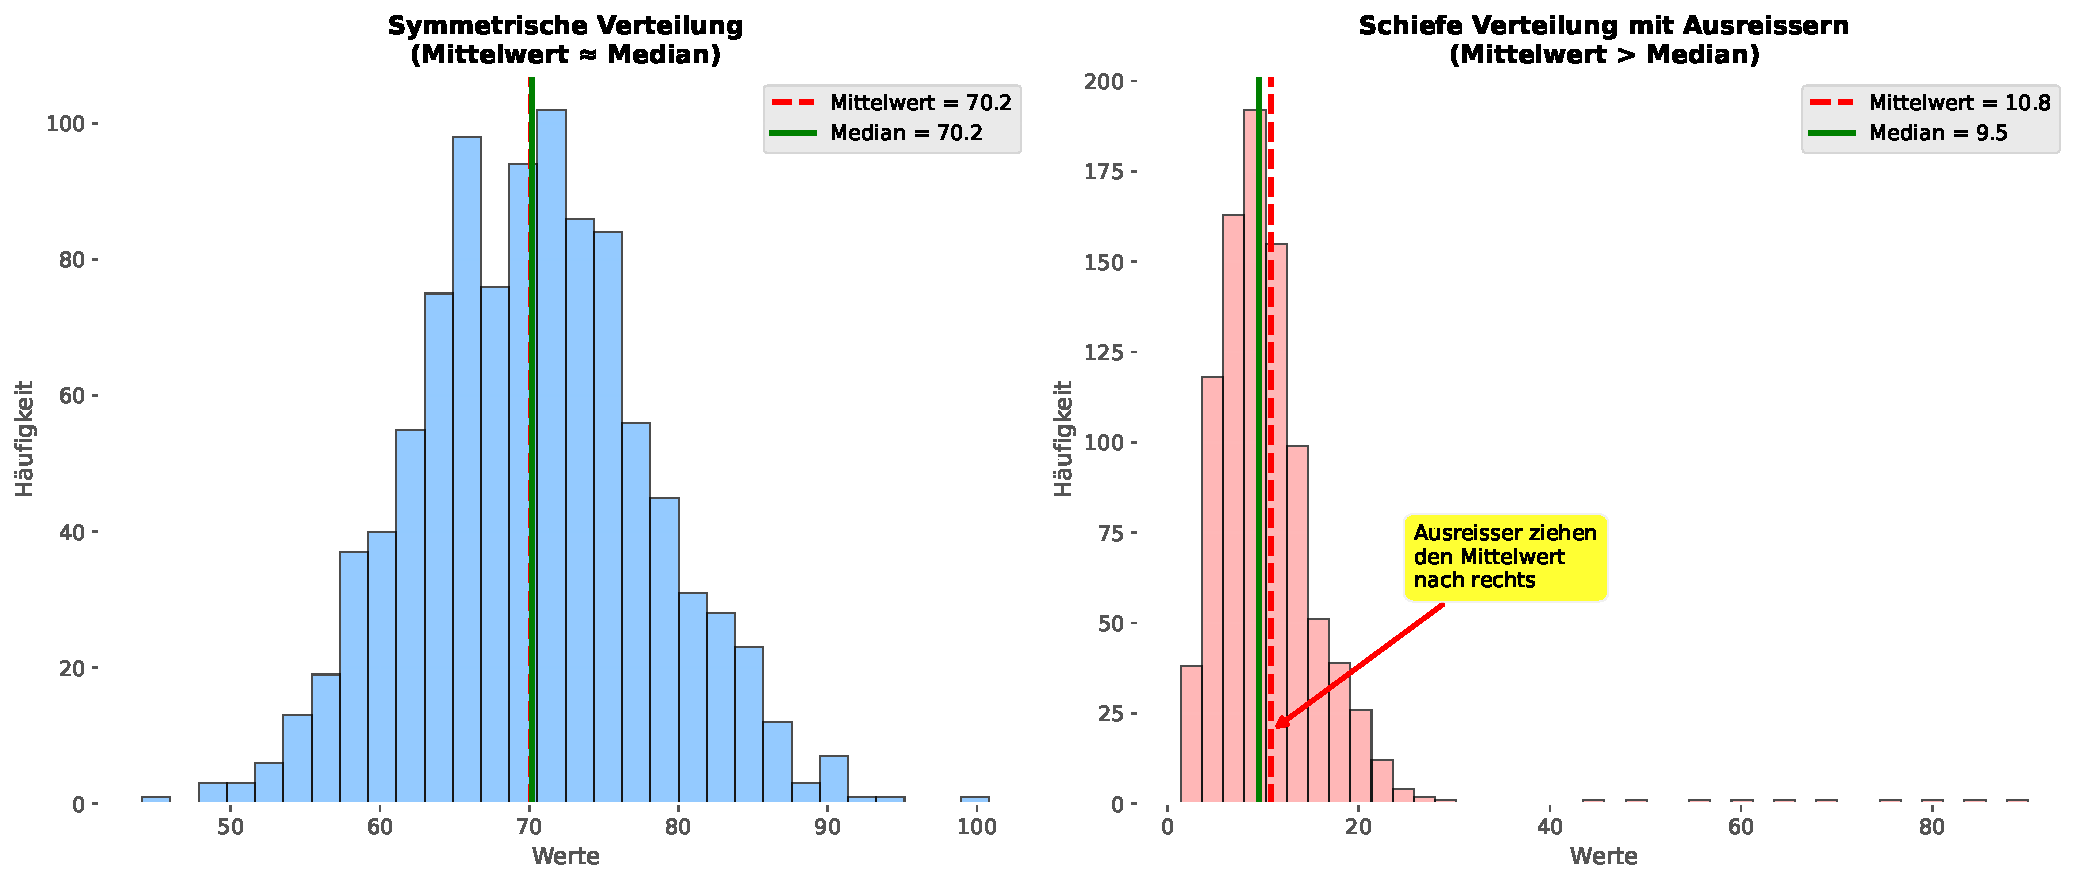
\includegraphics[width=0.95\textwidth]{Various/Wahlpflichtmodul Statistik/Figures/plots_mean_vs_median.pdf}
	\caption{Vergleich: Mittelwert und Median bei symmetrischer vs. schiefer Verteilung}
	\label{fig:mean_vs_median}
\end{figure}

\begin{myexercise}\label{myexercise:median-mean-ausreisser}
	Betrachten Sie die Daten (z.B.\ monatliches Taschengeld in \gls{CHF}):
	\[
		20,\ 25,\ 25,\ 30,\ 30,\ 35,\ 40,\ 400.
	\]
	\begin{enumerate}
		\item Bestimmen Sie den Median.
		\item Schätzen Sie den Mittelwert (grob reicht).
		\item Welche Kennzahl beschreibt das ``typische'' Taschengeld besser? Begründen Sie.
	\end{enumerate}
	\begin{myanswer}
		\begin{enumerate}
			\item Sortiert sind die Werte bereits. Median ist der Mittelwert des 4.\ und 5.\ Wertes: $(30+30)/2=30$.
			\item Mittelwert: Summe $=605$, geteilt durch $8$ ergibt ca.\ $75.6$.
			\item Median, weil der Ausreisser $400$ den Mittelwert stark nach oben zieht.
		\end{enumerate}
	\end{myanswer}
\end{myexercise}

\begin{figure}[H]
	\centering
	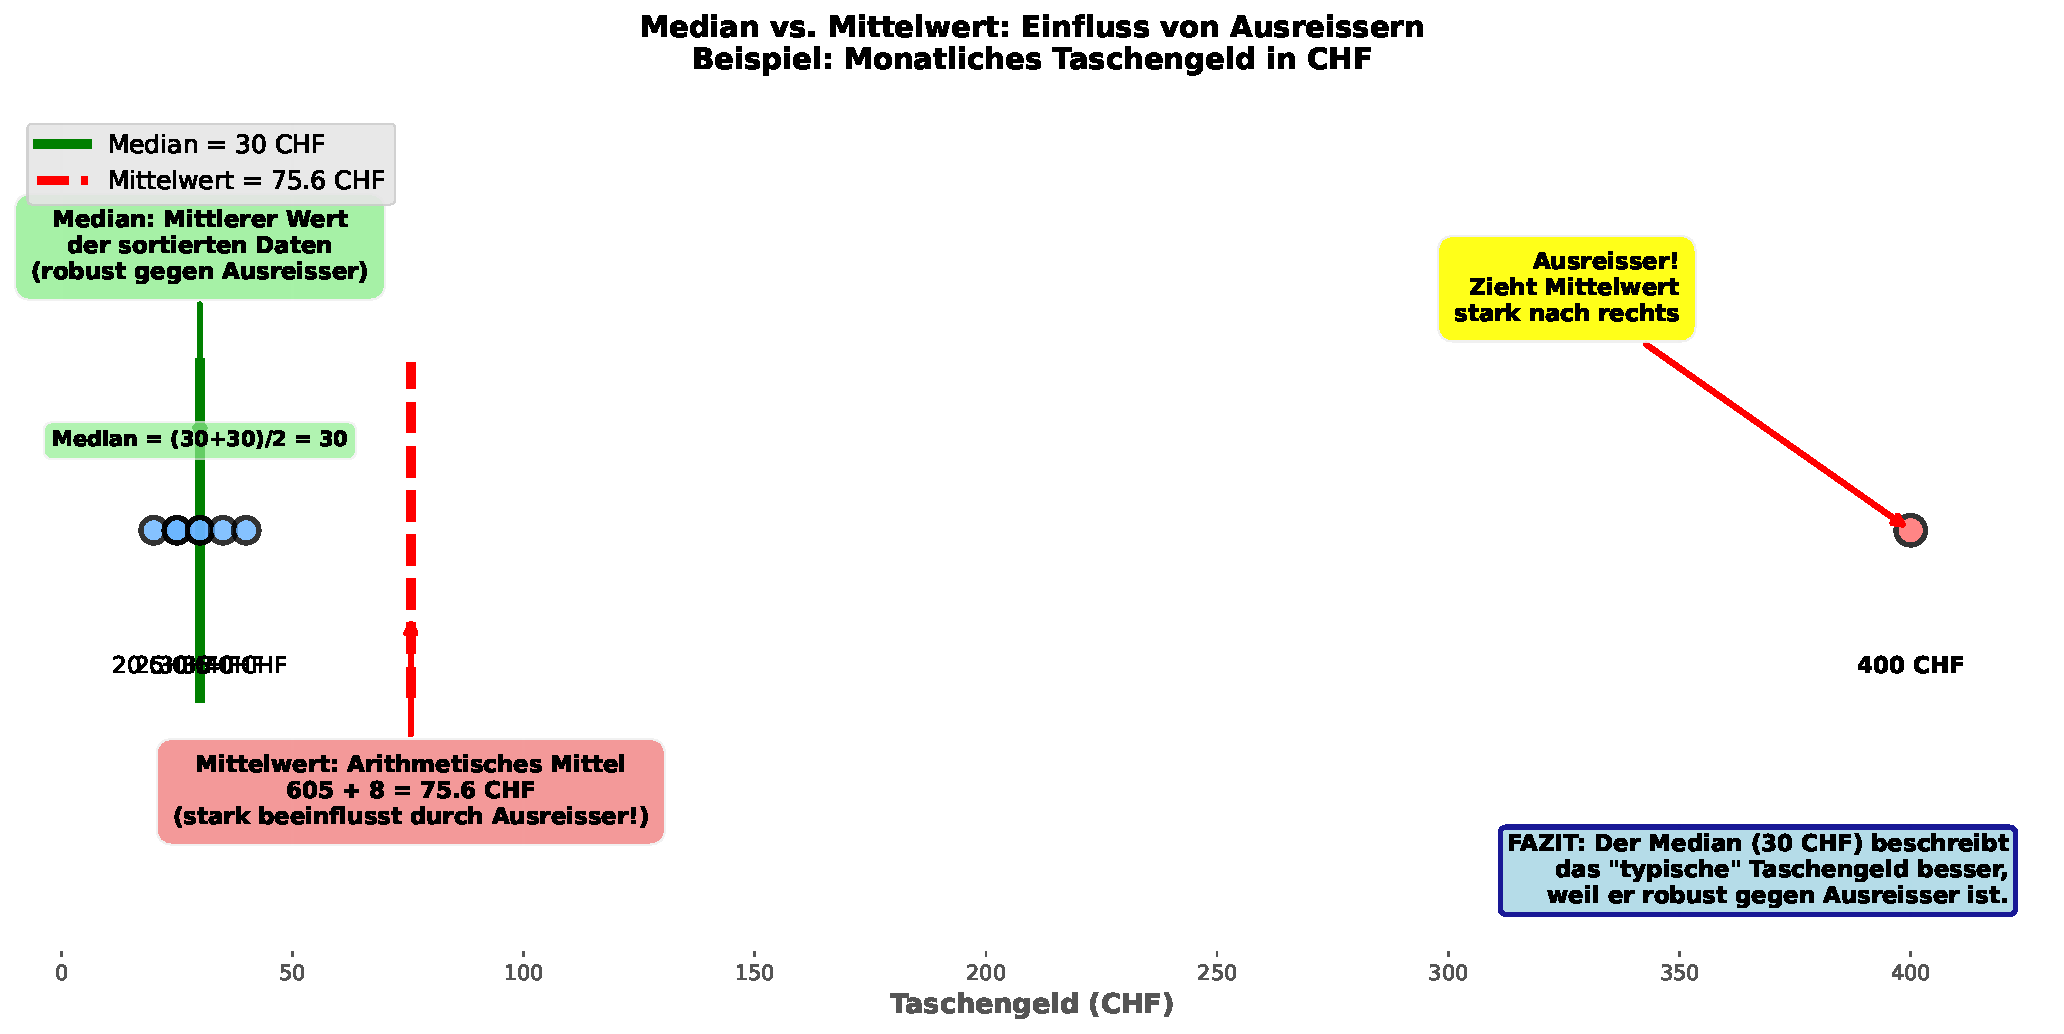
\includegraphics[width=0.95\textwidth]{Various/Wahlpflichtmodul Statistik/Figures/plots_median_calculation.pdf}
	\caption{Visualisierung der Median-Berechnung und des Ausreisser-Effekts}
	\label{fig:median_calculation}
\end{figure}

\subsection{Streuung}
Streuung beschreibt, wie stark Daten um die zentrale Lage variieren.

\begin{mydefinition}\label{mydefinition:spannweite}
	Die \textbf{Spannweite} einer Verteilung ist definiert als $\max(x)-\min(x)$. Diese Metrik ist sehr anfällig für Ausreisser, da sie nur die Extremwerte betrachtet.
\end{mydefinition}

\begin{mydefinition}\label{mydefinition:quartile-iqr}
	\textbf{Quartile:} $Q1$ ist das 25\%-Quantil, $Q3$ das 75\%-Quantil. Quartile teilen die Daten in vier gleich grosse Teile. Damit dies möglich ist, müssen die Daten sortiert werden. Damit Daten überhaupt sortierbar sind, müssen sie mindestens auf einer Ordinalskala vorliegen.

	Der \textbf{\acrfull{IQR}} ist $Q3-Q1$. Dieser wird häufig verwendet, um die Streuung zu beschreiben, da er robust gegenüber Ausreissern ist.
\end{mydefinition}

\begin{figure}[H]
	\centering
	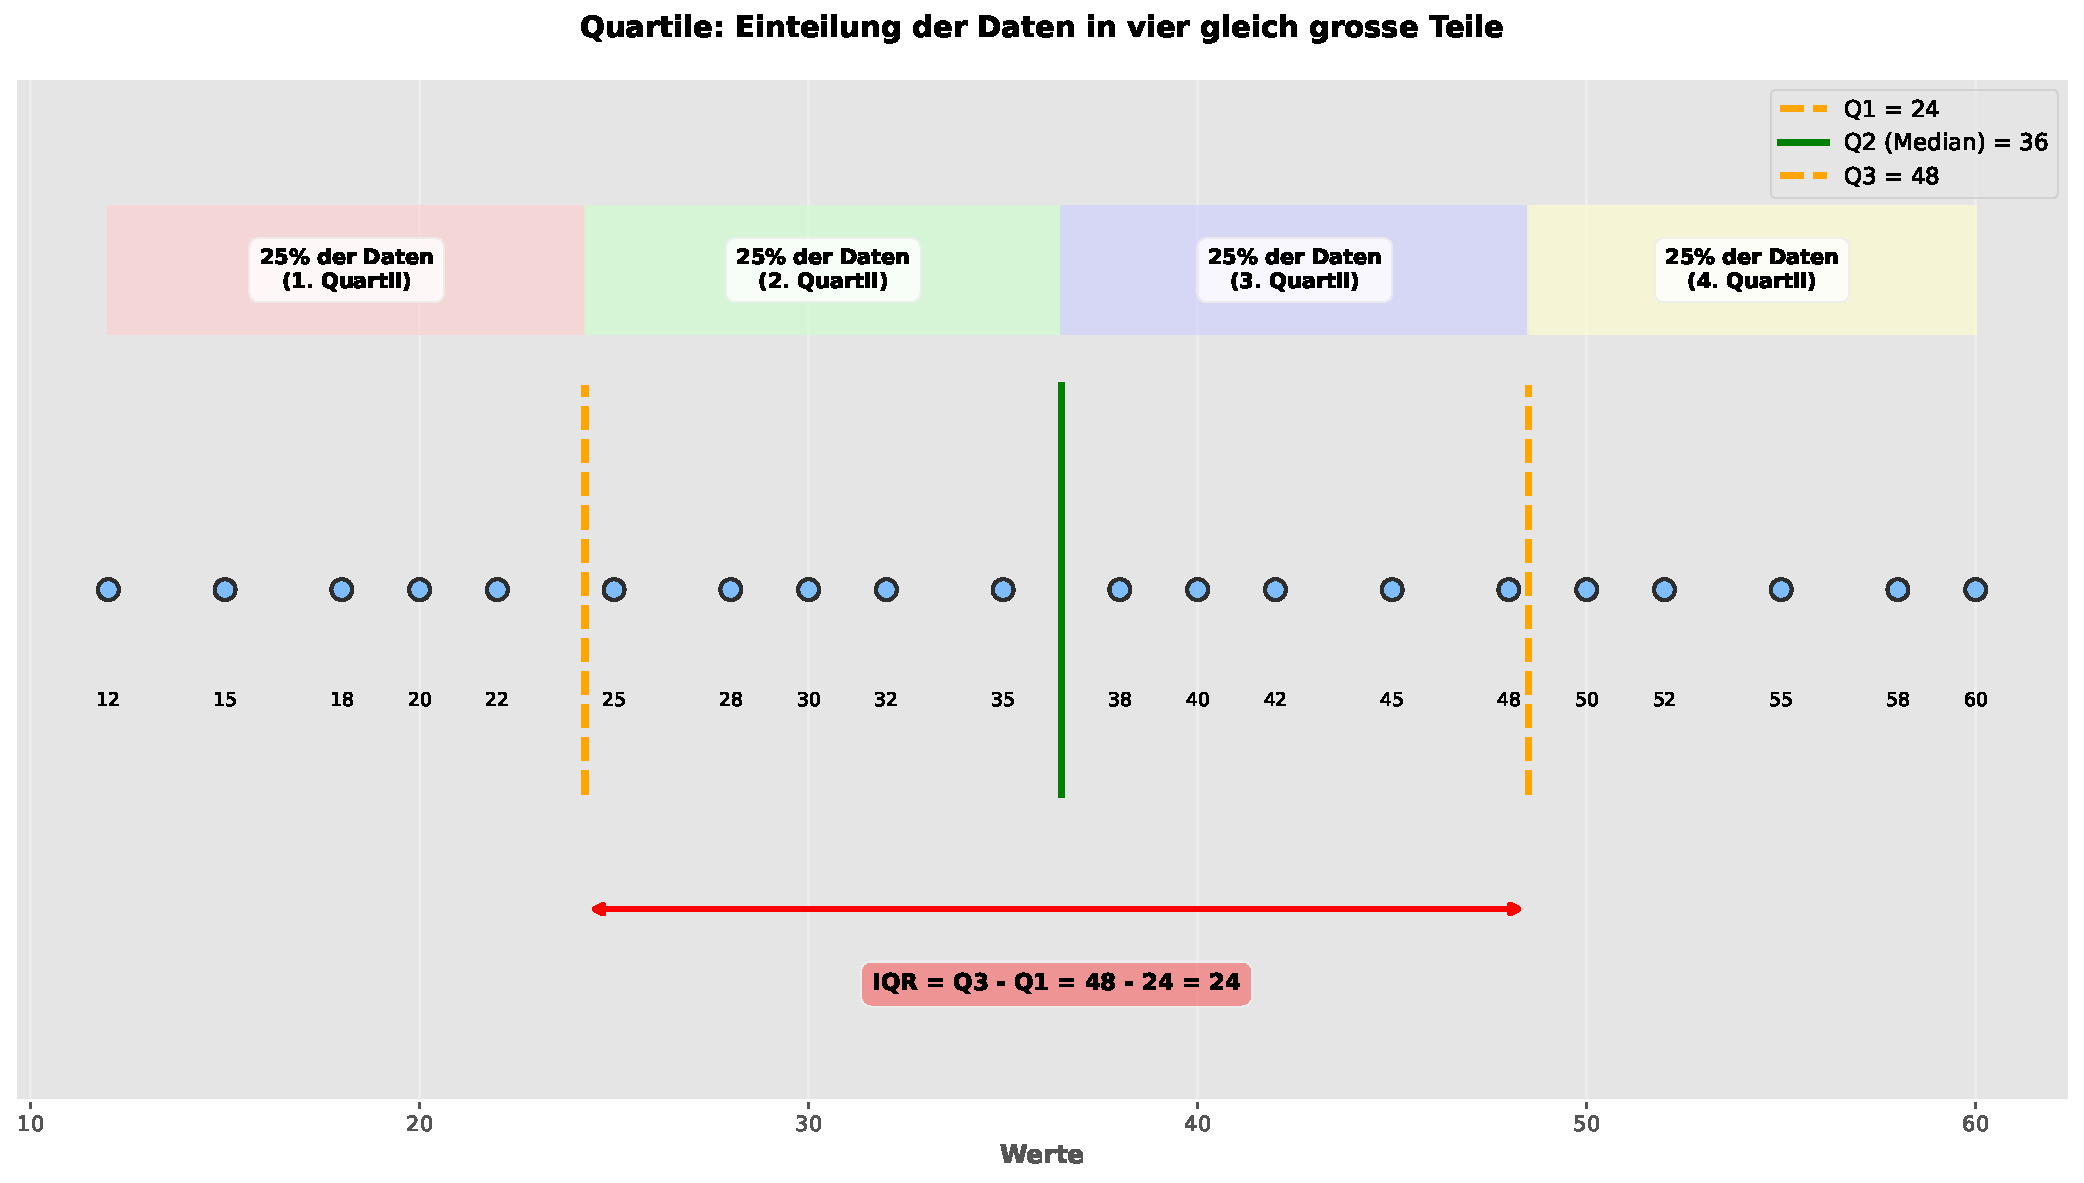
\includegraphics[width=0.95\textwidth]{Various/Wahlpflichtmodul Statistik/Figures/plots_quartiles.pdf}
	\caption{Quartile teilen die sortierten Daten in vier gleich grosse Teile}
	\label{fig:quartiles}
\end{figure}

\begin{mydefinition}\label{mydefinition:standardabweichung}
	Die \textbf{Standardabweichung} (Stichprobe) ist
	\[
		s=\sqrt{\frac{1}{n-1}\sum_{i=1}^{n}(x_i-\bar{x})^2}.
	\]
	Wobei $\bar{x}$ der Mittelwert der Daten ist. Die Standardabweichung misst also die durchschnittliche Abweichung der Daten vom Mittelwert. Sie ist jedoch empfindlich gegenüber Ausreissern, da diese den Mittelwert stark beeinflussen können.
\end{mydefinition}

\begin{figure}[H]
	\centering
	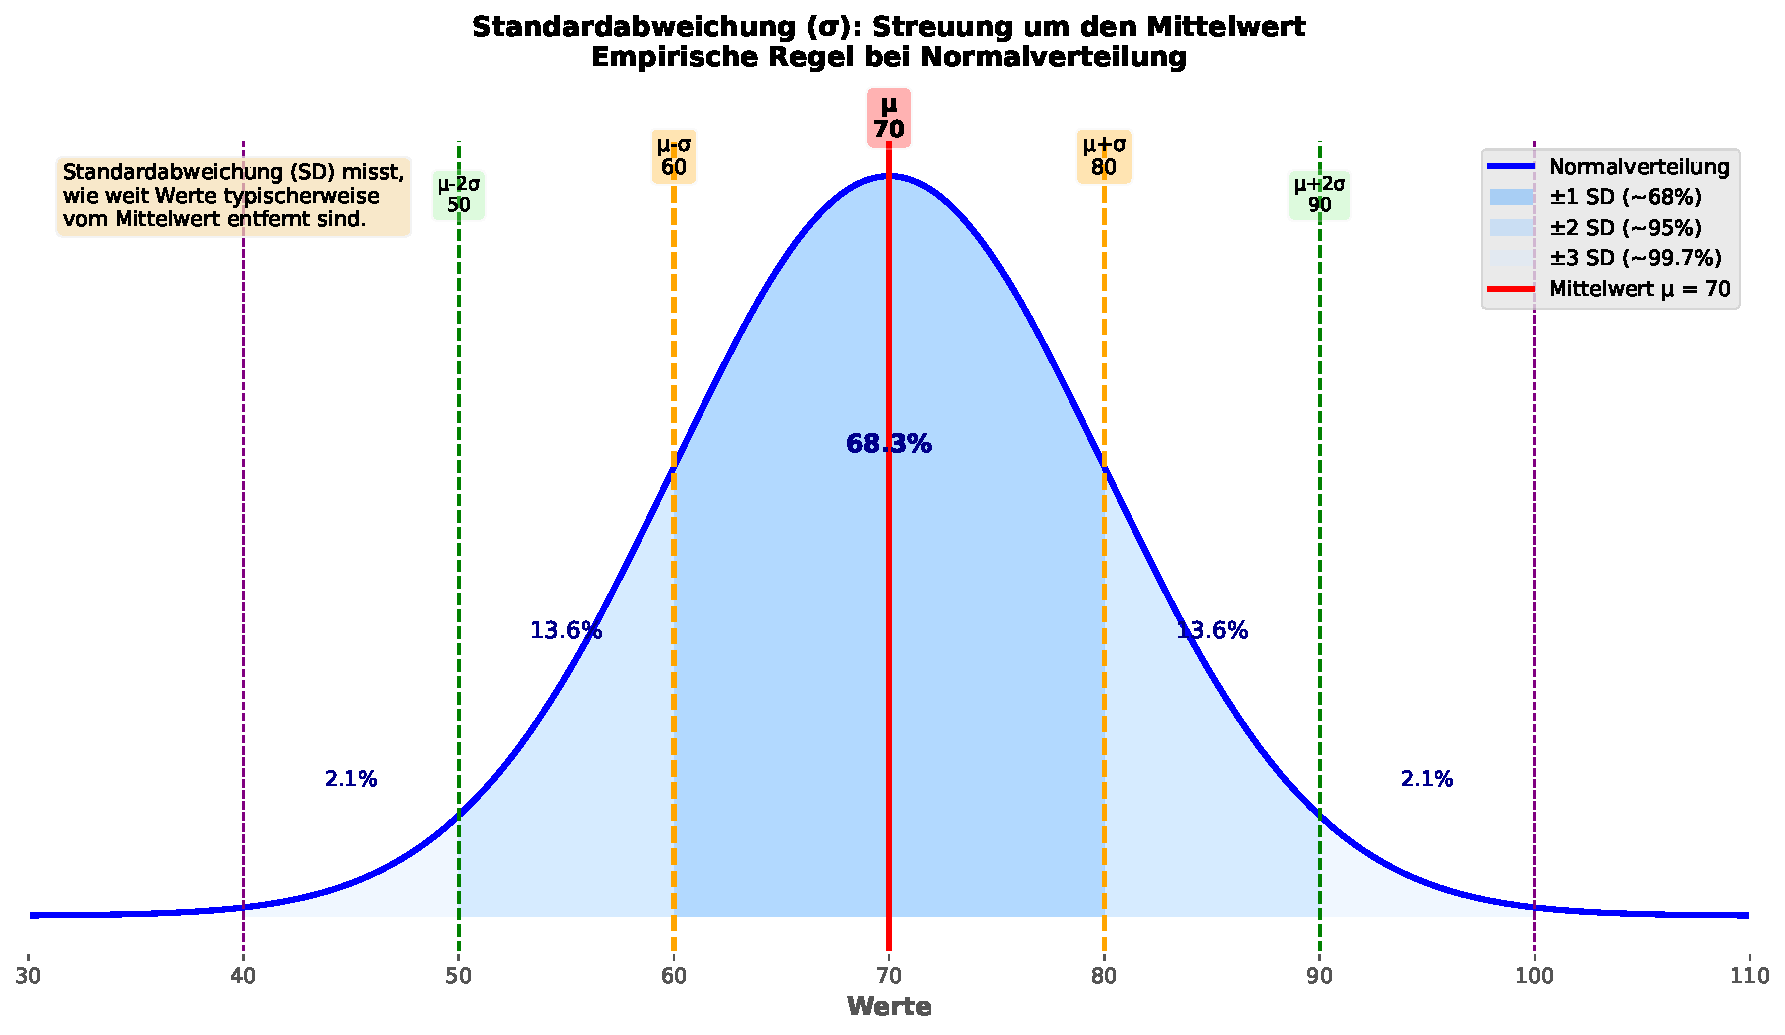
\includegraphics[width=0.9\textwidth]{Various/Wahlpflichtmodul Statistik/Figures/plots_standard_deviation.pdf}
	\caption{Standardabweichung: Streuung um den Mittelwert bei Normalverteilung}
	\label{fig:standard_deviation}
\end{figure}

\begin{myremark}
	Typische Paarung:
	\begin{itemize}
		\item \textbf{Median} zusammen mit \textbf{\gls{IQR}}
		\item \textbf{Mittelwert} zusammen mit \textbf{Standardabweichung}
	\end{itemize}
\end{myremark}

\section{Darstellungen: Tabelle, Text, Grafik}

\subsection{Welche Darstellung wofür?}

\begin{mydefinition}[Text und Tabellen]
	Text und Tabellen sind ideal, um genaue Werte zu kommunizieren (z.B.\ Mittelwert = 7.2 Stunden) oder um kleine Stichproben übersichtlich darzustellen.

	\textbf{Beispiel:} Ein Artikel berichtet: ``Die durchschnittliche Schlafdauer beträgt 7.2 Stunden (\gls{SD} = 1.5).'' Hier werden genaue Werte kommuniziert, die in Textform gut verständlich sind.

	Ein anderes Beispiel: Eine Tabelle zeigt die Schlafdauer von 3 Personen. Hier ist die tabellarische Darstellung übersichtlicher als eine Grafik, da es sich um wenige Datenpunkte handelt.

	\begin{table}[H]
		\centering
		\caption{Beispiel einer Tabelle mit Schlafdaten von 3 Personen}
		\begin{tabular}{c c}
			\toprule
			\textbf{Person} & \textbf{Schlafdauer (Stunden)} \\
			\midrule
			A               & 7.0                            \\
			B               & 6.5                            \\
			C               & 8.0                            \\
			\bottomrule
		\end{tabular}
	\end{table}
\end{mydefinition}

\begin{mydefinition}[Balken- und Kreisdiagramme]
	Balken- und Kreisdiagramme sind geeignet, um Verhältnisse zwischen Kategorien darzustellen. Sie eignen sich besonders gut, wenn die Kategorien nominal skaliert sind.

	\begin{figure}[H]
		\centering
		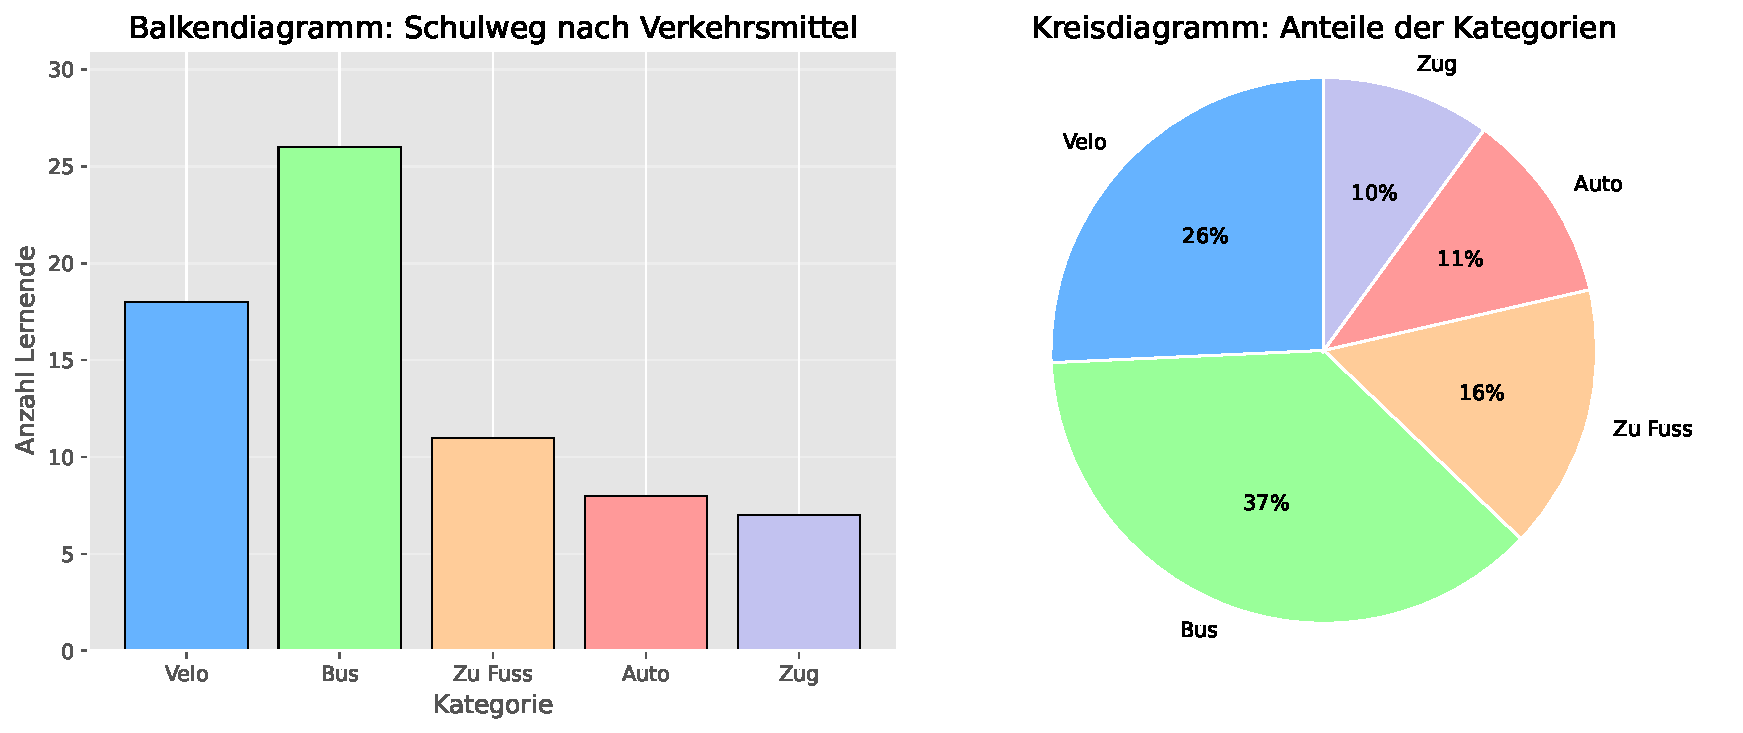
\includegraphics[width=0.95\textwidth]{Various/Wahlpflichtmodul Statistik/Figures/plots_bar_pie.pdf}
		\caption{Beispiel eines Balkendiagramms und eines Kreisdiagramms}
	\end{figure}

	Balkendiagramme können auch für ordinal oder intervallskalierte Daten verwendet werden und eignen sich besser, wenn die Kategorien viele Werte haben oder wenn genaue Werte kommuniziert werden sollen. Kreisdiagramme sollten nur bei wenigen Kategorien verwendet werden, da sie bei vielen Kategorien unübersichtlich werden können.
\end{mydefinition}

\begin{mydefinition}[Scatterplot]
	Ein \textbf{Scatterplot} zeigt die Beziehung zwischen zwei metrischen Variablen (z.B.\ Schlafdauer und Fokus-Score), indem jeder Datenpunkt als Punkt in einem Koordinatensystem dargestellt wird. Er eignet sich besonders gut, um Korrelationen oder Muster in den Daten zu erkennen.
	\begin{figure}[H]
		\centering
		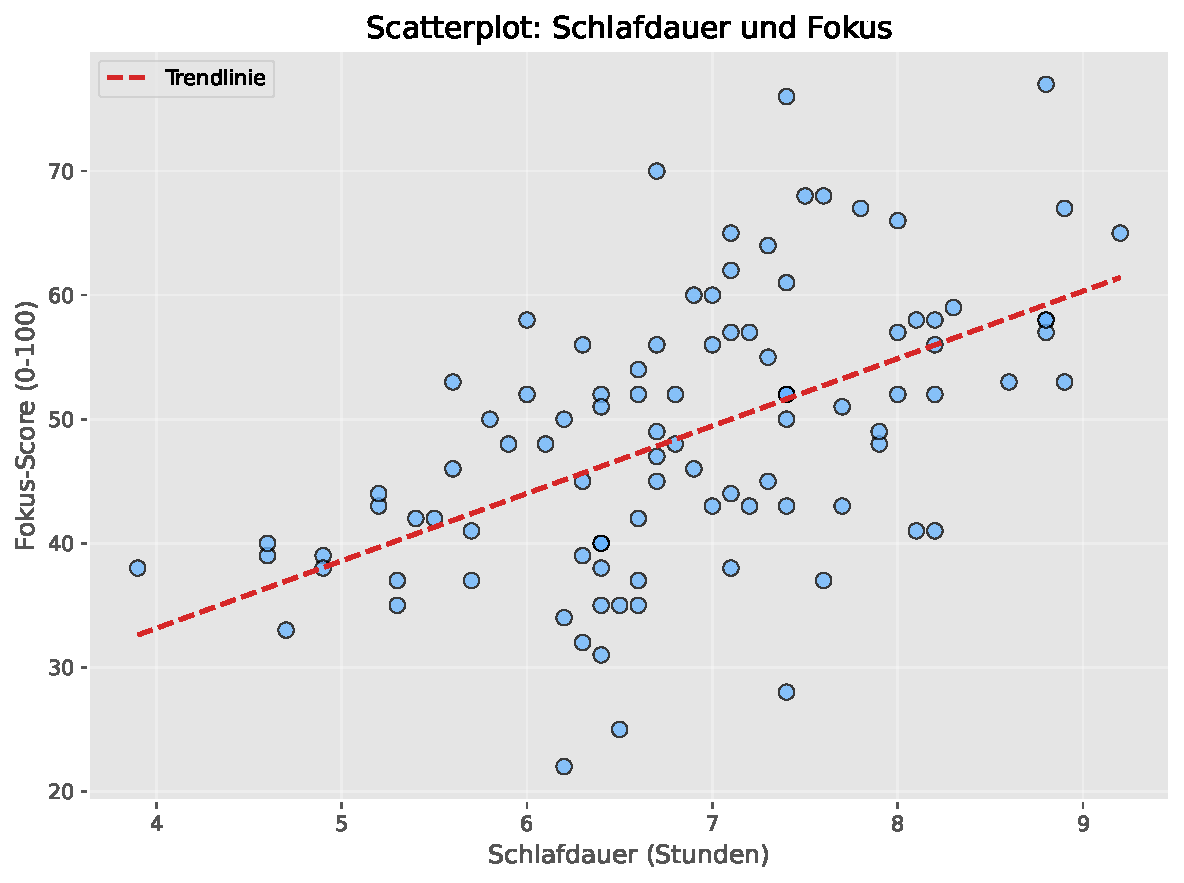
\includegraphics[width=0.75\textwidth]{Various/Wahlpflichtmodul Statistik/Figures/plots_scatterplot.pdf}
		\caption{Beispiel eines Scatterplots: Schlafdauer und Fokus-Score}
		\label{fig:scatterplot_sleep_focus}
	\end{figure}
\end{mydefinition}

\begin{mydefinition}[Histogramm]
	Ein \textbf{Histogramm} zeigt die Verteilung einer metrischen Variable (z.B.\ Schlafdauer), indem es die Häufigkeit (oder relative Häufigkeit) von Werten in bestimmten Intervallen (Bins) darstellt. Es eignet sich besonders gut, um die Form der Verteilung zu erkennen (z.B.\ Schiefe, Modus, Ausreisser).

	\begin{figure}[H]
		\centering
		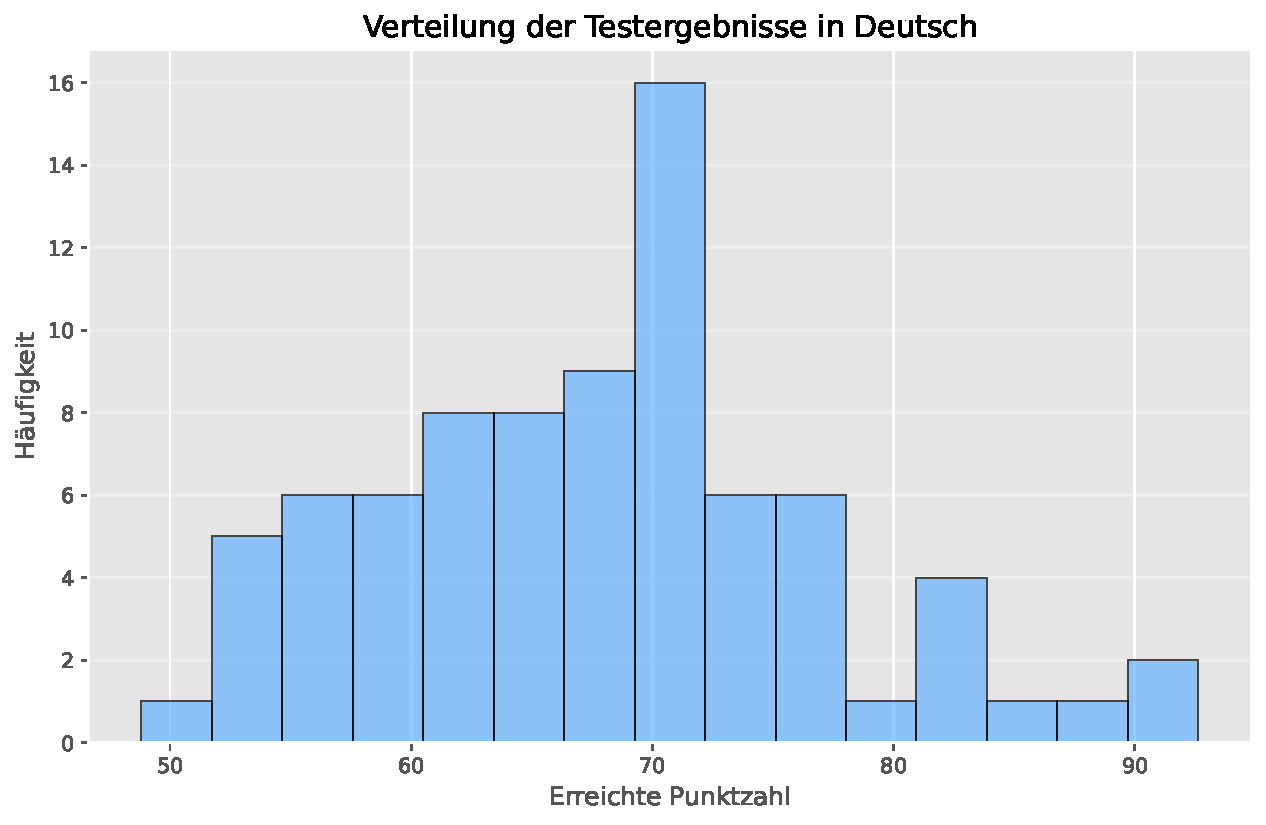
\includegraphics[width=0.6\textwidth]{Various/Wahlpflichtmodul Statistik/Figures/plots_histogram.pdf}
		\caption{Beispiel eines Histogramms}
	\end{figure}
\end{mydefinition}

\begin{mydefinition}[Boxplot]
	Ein \textbf{Boxplot} (Kastendiagramm) visualisiert die Verteilung einer metrischen Variable durch:
	\begin{itemize}
		\item Eine Box von $Q1$ bis $Q3$ (Interquartilsabstand)
		\item Eine Linie im Inneren der Box für den Median
		\item ``Whiskers'' (Antennen) bis zum letzten Wert innerhalb von $1.5 \times$ \gls{IQR} von den Quartilen
		\item Punkte für Ausreisser, die ausserhalb der Whiskers liegen
	\end{itemize}
	\begin{figure}[H]
		\centering
		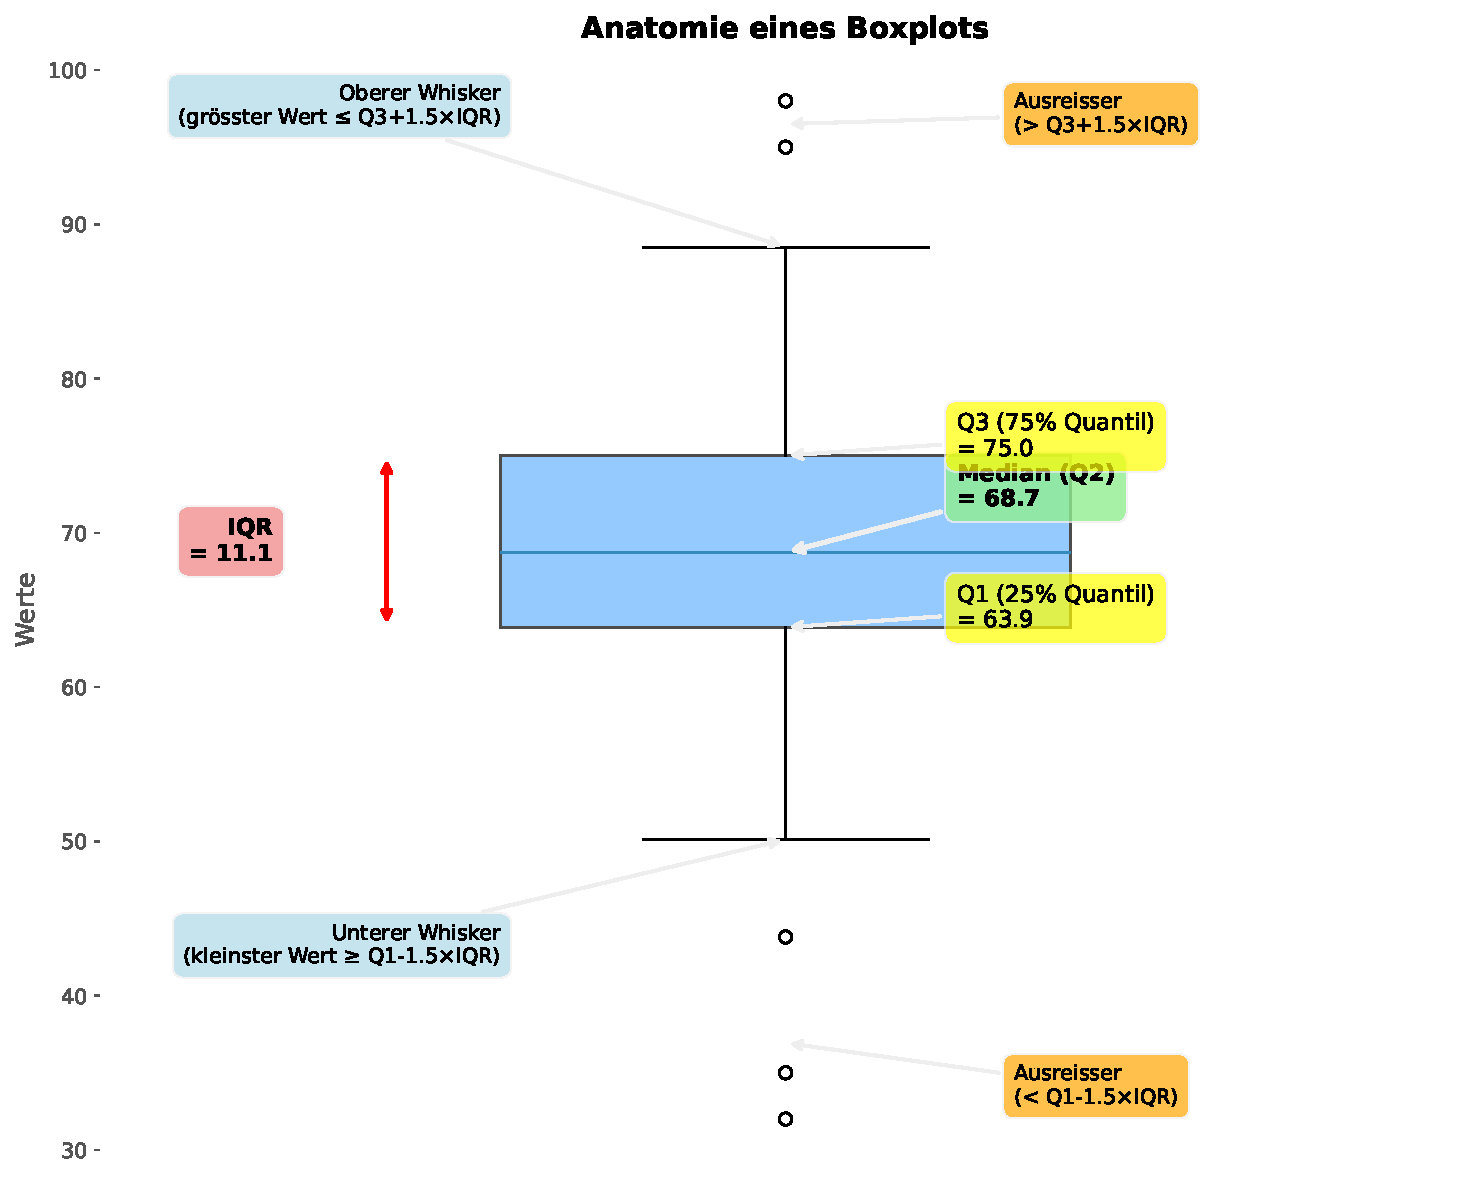
\includegraphics[width=0.85\textwidth]{Various/Wahlpflichtmodul Statistik/Figures/plots_boxplot_anatomy.pdf}
		\caption{Anatomie eines Boxplots: Alle Komponenten erklärt}
		\label{fig:boxplot_anatomy}
	\end{figure}
\end{mydefinition}

\subsection{Formen von Verteilungen (reduziert)}

\begin{figure}[H]
	\centering
	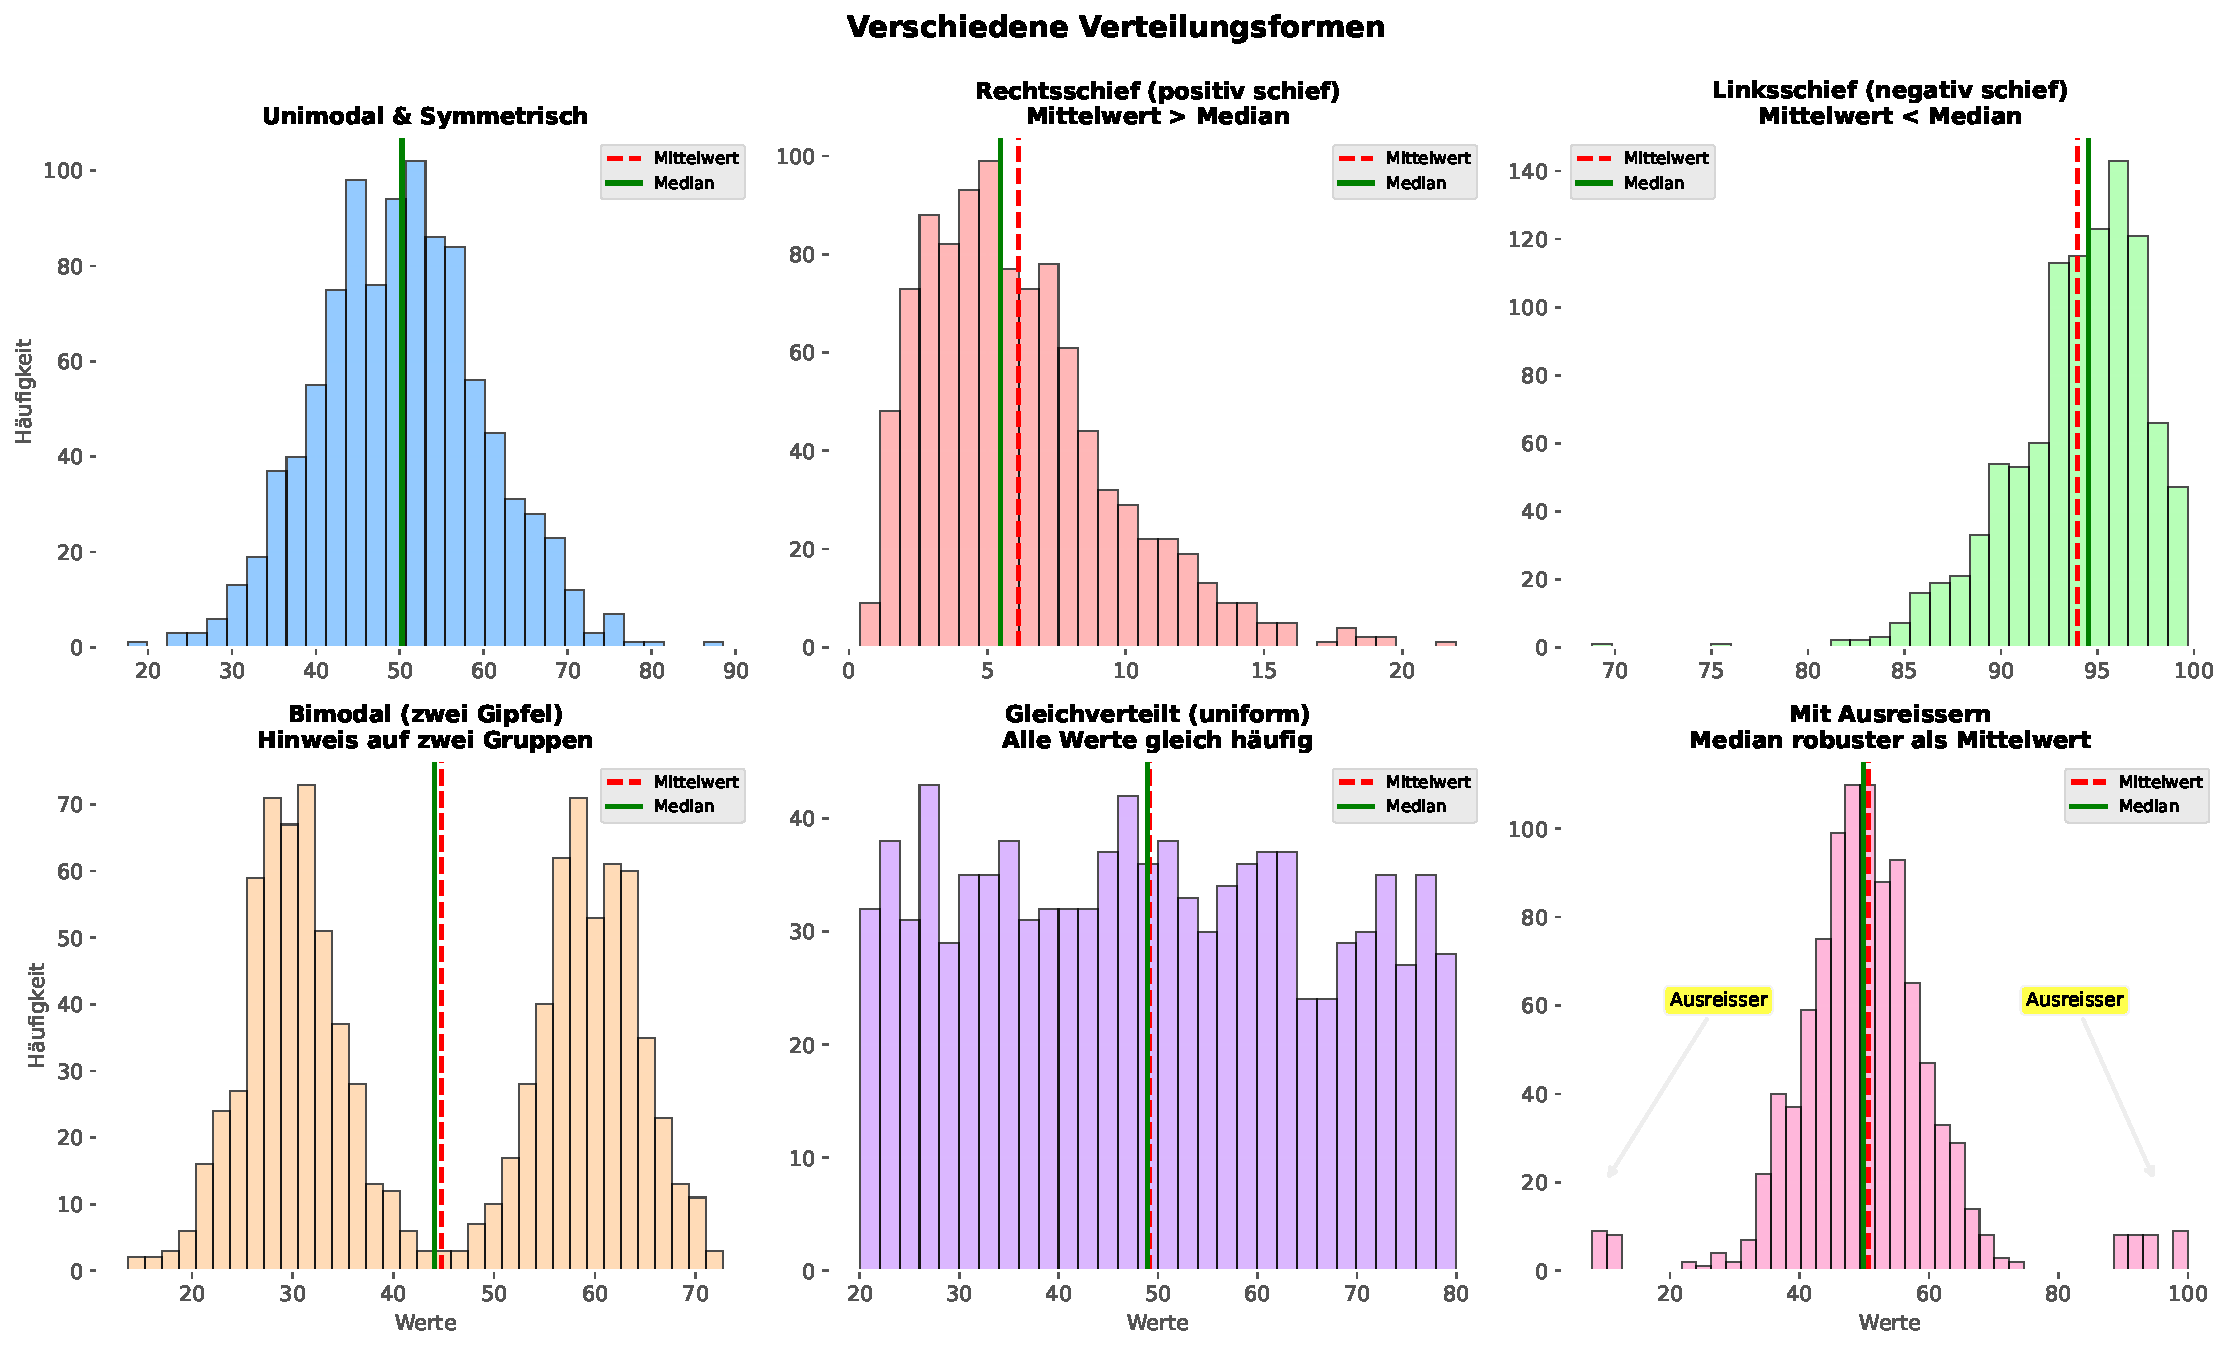
\includegraphics[width=0.95\textwidth]{Various/Wahlpflichtmodul Statistik/Figures/plots_distribution_shapes.pdf}
	\caption{Verschiedene Verteilungsformen und ihre Eigenschaften}
	\label{fig:distribution_shapes}
\end{figure}

\begin{myremark}
	Für dieses Modul fokussieren wir auf wenige, aber zentrale Formen:
	\begin{itemize}
		\item \textbf{Symmetrisch}: Mittelwert $\approx$ Median
		\item \textbf{Rechtsschief}: Wenige hohe Ausreisser, Mittelwert $>$ Median
	\end{itemize}
	Die weiteren Formen (z.B. linkschief, bimodal) sind möglich, stehen aber nicht im Zentrum.

	Für die Praxis genügt häufig die Entscheidung:
	\begin{itemize}
		\item eher symmetrisch $\Rightarrow$ Mittelwert + \gls{SD}
		\item deutlich schief $\Rightarrow$ Median + \gls{IQR}
	\end{itemize}
\end{myremark}

\subsection{Kritisches Lesen von Grafiken}
\begin{myattention}
	Beim Lesen von Grafiken immer prüfen:
	\begin{itemize}
		\item Startet die Achse bei 0 (Gefahr von Verzerrung)?
		\item Sind Kategorien gleich breit (Gefahr von visueller Überinterpretation einzelner Kategorien)?
		\item Fehlen Werte oder Gruppen (Gefahr von inhaltlichen Interpretationen)?
	\end{itemize}
\end{myattention}

\begin{myexercise}\label{myexercise:grafik-checkliste}
	Eine Zeitung zeigt ein Balkendiagramm: Die y-Achse startet bei 60 statt bei 0.

	\begin{figure}[H]
		\centering
		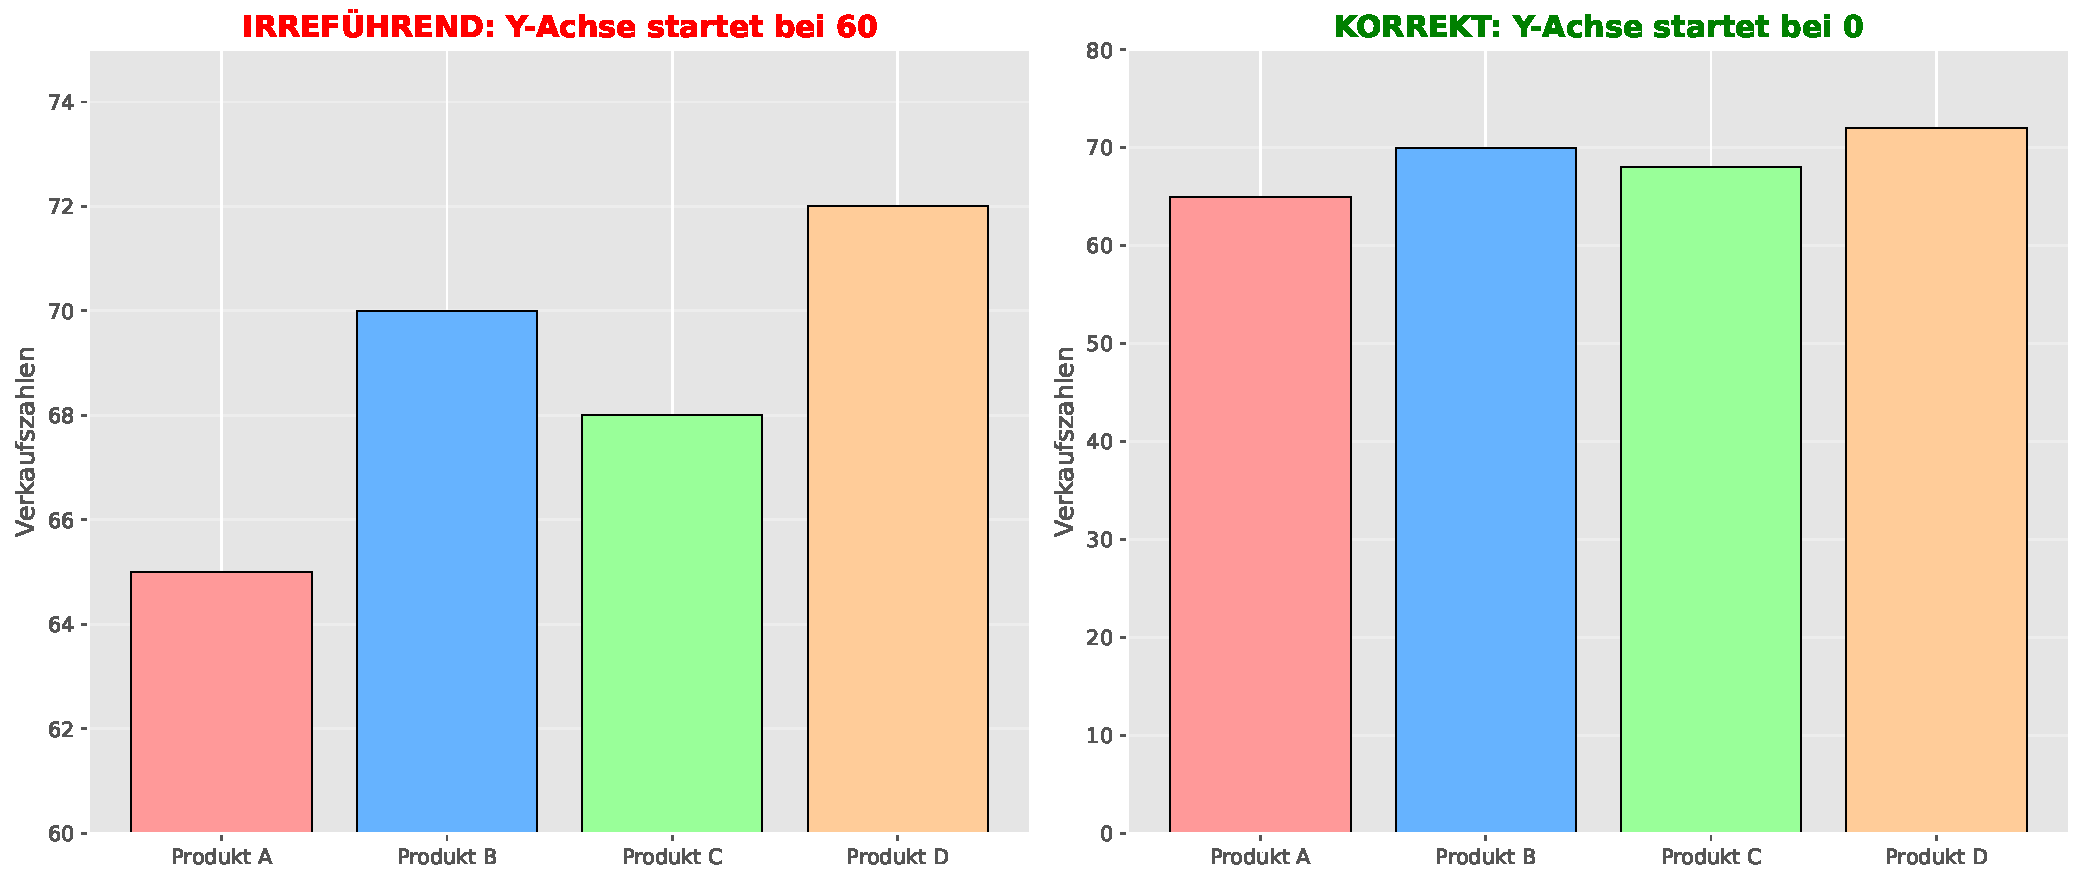
\includegraphics[width=0.95\textwidth]{Various/Wahlpflichtmodul Statistik/Figures/plots_misleading_axes.pdf}
		\caption{Vergleich: Irreführende vs. korrekte Darstellung der Y-Achse}
	\end{figure}

	\begin{enumerate}
		\item Welchen Effekt hat das auf die Wirkung der Grafik?
		\item Formulieren Sie eine sachliche Kritik in einem Satz.
	\end{enumerate}
	\begin{myanswer}
		\begin{enumerate}
			\item Unterschiede wirken viel grösser und dramatischer als sie tatsächlich sind.
			\item ``Da die y-Achse nicht bei 0 startet, werden die Unterschiede optisch übertrieben dargestellt.''
		\end{enumerate}
	\end{myanswer}
\end{myexercise}

\section{Arbeiten mit \texorpdfstring{\gls{CODAP}}{CODAP} und Datensätzen}

\subsection{Datensatz bereitstellen}
Sie erhalten zwei Datensätze als \gls{CSV}-Dateien, die Sie (oder Ihre Lehrperson) bereitstellen:
\begin{itemize}
	\item \texttt{sleep\_focus.csv} (Schlaf, Smartphone, Stress, Fokus)
	\item \texttt{music\_study.csv} (optional: Kontingenztabelle, siehe Challenge)
\end{itemize}

\begin{myattention}
	Import in \gls{CODAP}: \href{https://codap.concord.org/app/static/dg/de/cert/index.html}{\texttt{codap.concord.org}} $\rightarrow$ Oben links $\rightarrow$ Öffnen $\rightarrow$ Lokale Datei.
\end{myattention}

\subsection{Datensatz 1: Schlaf und Fokus}
Der Datensatz \texttt{sleep\_focus.csv} enthält pro Person:
\begin{itemize}
	\item \texttt{SleepHours} (Stunden Schlaf)
	\item \texttt{PhoneMinutes} (Smartphone-Minuten)
	\item \texttt{Coffee} (0--4, ordinal)
	\item \texttt{Stress} (1--5, ordinal)
	\item \texttt{FocusScore} (Punktzahl 0--100)
\end{itemize}

\begin{table}[H]
	\centering
	\caption{Beispiel: Erste Zeilen des Datensatzes \texttt{sleep\_focus.csv}}
	\small
	\begin{tabular}{c c c c c c}
		\toprule
		\textbf{Person} & \textbf{SleepHours} & \textbf{PhoneMinutes} & \textbf{Coffee} & \textbf{Stress} & \textbf{FocusScore} \\
		\midrule
		1               & 7.5                 & 120                   & 2               & 3               & 78                  \\
		2               & 6.0                 & 200                   & 3               & 4               & 62                  \\
		3               & 8.2                 & 45                    & 1               & 2               & 85                  \\
		4               & 5.5                 & 310                   & 4               & 5               & 54                  \\
		5               & 7.0                 & 150                   & 2               & 3               & 72                  \\
		\dots           & \dots               & \dots                 & \dots           & \dots           & \dots               \\
		\bottomrule
	\end{tabular}
	\label{table:sleep_focus_example}
\end{table}

\subsection{Aufgabenpaket}

\begin{myexercise}\label{myexercise:aufgabenpaket-1}
	\textbf{Teil A: Kennzahlen (Einzelarbeit)} \\
	Arbeiten Sie mit \texttt{sleep\_focus.csv}.
	\begin{enumerate}
		\item Bestimmen Sie für \texttt{SleepHours} Median, Mittelwert, Minimum und Maximum.
		\item Entscheiden Sie: Würden Sie für \texttt{PhoneMinutes} eher Median oder Mittelwert berichten? Begründen Sie.
		\item Nennen Sie eine Situation, in der der Mittelwert sinnvoll ist, und eine, in der der Median sinnvoller ist.
	\end{enumerate}
	\begin{myanswer}
		\begin{enumerate}
			\item Werte in \gls{CODAP} ablesen (je nach Anzeige). Wichtig ist die Interpretation: typische Schlafdauer liegt im Bereich um 7 Stunden; Minimum/Maximum zeigen Spannweite.
			\item Eher Median, weil einzelne sehr hohe Nutzungszeiten den Mittelwert stark beeinflussen können.
			\item Mittelwert: symmetrische, ausreisserarme Daten (z.B.\ Körpergrössen). Median: schiefe Verteilungen oder Ausreisser (z.B.\ Einkommen).
		\end{enumerate}
	\end{myanswer}
\end{myexercise}

\begin{myexercise}\label{myexercise:aufgabenpaket-2}
	\textbf{Teil B: Visualisierung und Interpretation (Partnerarbeit)}
	\begin{enumerate}
		\item Erstellen Sie ein Histogramm von \texttt{SleepHours}. Beschreiben Sie die Verteilung (unimodal? schief? Ausreisser?).
		\item Erstellen Sie einen Boxplot von \texttt{PhoneMinutes}. Notieren Sie Q1, Median und Q3 (oder lesen Sie sie ab).
		\item Erstellen Sie einen Scatterplot \texttt{SleepHours} vs \texttt{FocusScore}. Formulieren Sie eine vorsichtige Aussage in einem Satz.
	\end{enumerate}
	\begin{myanswer}
		\begin{enumerate}
			\item Unimodal, die meisten Werte zwischen etwa 6 und 8 Stunden, einzelne kurze Nächte als Randwerte.
			\item Q1/Median/Q3 je nach \gls{CODAP}-Ablesung; wichtig: \gls{IQR} beschreibt typische Streuung ohne Ausreisser.
			\item ``Im Datensatz zeigt sich tendenziell: Wer mehr schläft, hat häufig einen höheren Fokus-Score; der Zusammenhang ist aber nicht perfekt.''
		\end{enumerate}
	\end{myanswer}
\end{myexercise}

\begin{myexample}
	\textbf{Beispiel einer Kontingenztabelle: Musik beim Lernen vs. Lernmodus}

	\begin{table}[H]
		\centering
		\begin{tabular}{l c c c}
			\toprule
			                    & \textbf{Alleine} & \textbf{Gruppe} & \textbf{Summe} \\
			\midrule
			\textbf{Mit Musik}  & 45 (56\%)        & 25 (31\%)       & 70             \\
			\textbf{Ohne Musik} & 35 (44\%)        & 55 (69\%)       & 90             \\
			\textbf{Summe}      & 80               & 80              & 160            \\
			\bottomrule
		\end{tabular}
		\caption{Beispiel einer Kontingenztabelle: Musik beim Lernen vs. Lernmodus}
		\label{table:kontingenztabelle}
	\end{table}

	Aus dieser Tabelle darf man z.B. beschreiben, welche Kombinationen in der Stichprobe häufiger vorkommen. Man darf daraus aber noch keine Ursache-Wirkung-Aussage ableiten.
\end{myexample}

\begin{mychallenge}\label{mychallenge:kontingenztabelle}
	\textbf{Challenge (optional): Kontingenztabelle} \\
	Arbeiten Sie mit der Kontingenztabelle aus dem Beispiel oben (ohne Computer).
	\begin{enumerate}
		\item Formulieren Sie zwei Aussagen, die durch die Tabelle gestützt werden.
		\item Formulieren Sie eine Aussage, die \textbf{nicht} zulässig ist, und begründen Sie kurz, warum.
	\end{enumerate}

	\begin{myanswer}
		Zulässig sind beschreibende Aussagen zur Stichprobe, z.B.\ ``In dieser Stichprobe lernen Personen ohne Musik häufiger in Gruppen als Personen mit Musik.''. Eine weitere zulässige Aussage könnte sein: ``Insgesamt lernen 70 Personen mit Musik, 90 Personen ohne Musik.''.

		Nicht zulässig sind kausale Aussagen wie ``Musik verbessert das Lernen.''
	\end{myanswer}
\end{mychallenge}

\section{Schliessende Statistik: Von der Stichprobe zur Aussage}

\subsection{Grundidee}
In der beschreibenden Statistik fassen wir genau die vorliegenden Daten zusammen.
In der schliessenden Statistik fragen wir zusätzlich:
\begin{center}
	\textit{Was sagen unsere Daten über eine grössere Grundgesamtheit aus?}
\end{center}

\begin{mydefinition}
	Eine \textbf{Stichprobe} ist die beobachtete Teilmenge.
	Die \textbf{Grundgesamtheit} ist die grössere Gruppe, über die wir Aussagen machen möchten.
\end{mydefinition}

\subsection{Vertrauensintervall als Basis statistischer Tests}

\begin{myremark}
	Ein Vertrauensintervall beschreibt einen plausiblen Bereich für einen unbekannten Wert.
	Je schmaler das Intervall, desto präziser ist die Aussage; je breiter das Intervall, desto grösser ist die Unsicherheit.
\end{myremark}

\begin{myexample}
	\textbf{Vollständig durchgerechnetes Beispiel (Gähn-Experiment)}

	Bedeutung der Symbole im Beispiel: $n$ ist die Anzahl Personen in einer Gruppe (Stichprobengrösse),
	$x$ ist die Anzahl Personen mit dem Ereignis (hier: gähnen),
	$\hat{p}=x/n$ ist der beobachtete Anteil in Prozent,
	$\hat{\Delta}=\hat{p}_{\mathrm{exp}}-\hat{p}_{\mathrm{kontr}}$ ist der beobachtete Unterschied zwischen Experimental- und Kontrollgruppe,
	und $\mathrm{SE}(\hat{\Delta})$ ist der Standardfehler, also ein Mass dafür, wie stark dieser Unterschied zufallsbedingt schwanken kann.

	Gegeben seien
	\[
		n_{\mathrm{exp}}=34,\quad x_{\mathrm{exp}}=10,
		\qquad
		n_{\mathrm{kontr}}=16,\quad x_{\mathrm{kontr}}=4.
	\]
	Damit folgt
	\[
		\hat{p}_{\mathrm{exp}}\approx29.4\%,
		\qquad
		\hat{p}_{\mathrm{kontr}}=25.0\%,
		\qquad
		\hat{\Delta}=29.4\%-25.0\%=4.4\text{ Prozentpunkte}.
	\]
	Für die Rechnung im Standardfehler verwenden wir die Anteile als Dezimalzahlen (also 0.294 und 0.25).

	Nun der \textbf{Standardfehler} der Differenz:
	\[
		\mathrm{SE}(\hat{\Delta})
		=\sqrt{\frac{0.294\cdot 0.706}{34}+\frac{0.25\cdot 0.75}{16}}
		=\sqrt{0.00610+0.01172}
		=\sqrt{0.01782}
		\approx 0.134.
	\]

	Das \textbf{95\%-Vertrauensintervall} für den Unterschied lässt sich nun berechnen als:
	\[
		0.044 \pm 1.96\cdot 0.134
		=0.044\pm 0.262
		\Rightarrow
		[-0.218,\,0.306]\approx[-21.8\%,\,30.6\%].
	\]

	Interpretation: 0 liegt im Intervall. Mit diesen Daten ist auf diesem Niveau kein klarer Unterschied zwischen den Gruppen nachweisbar. Folgende Grafik illustriert diese Aussage grafisch.
	
	\begin{figure}[H]
        \centering
        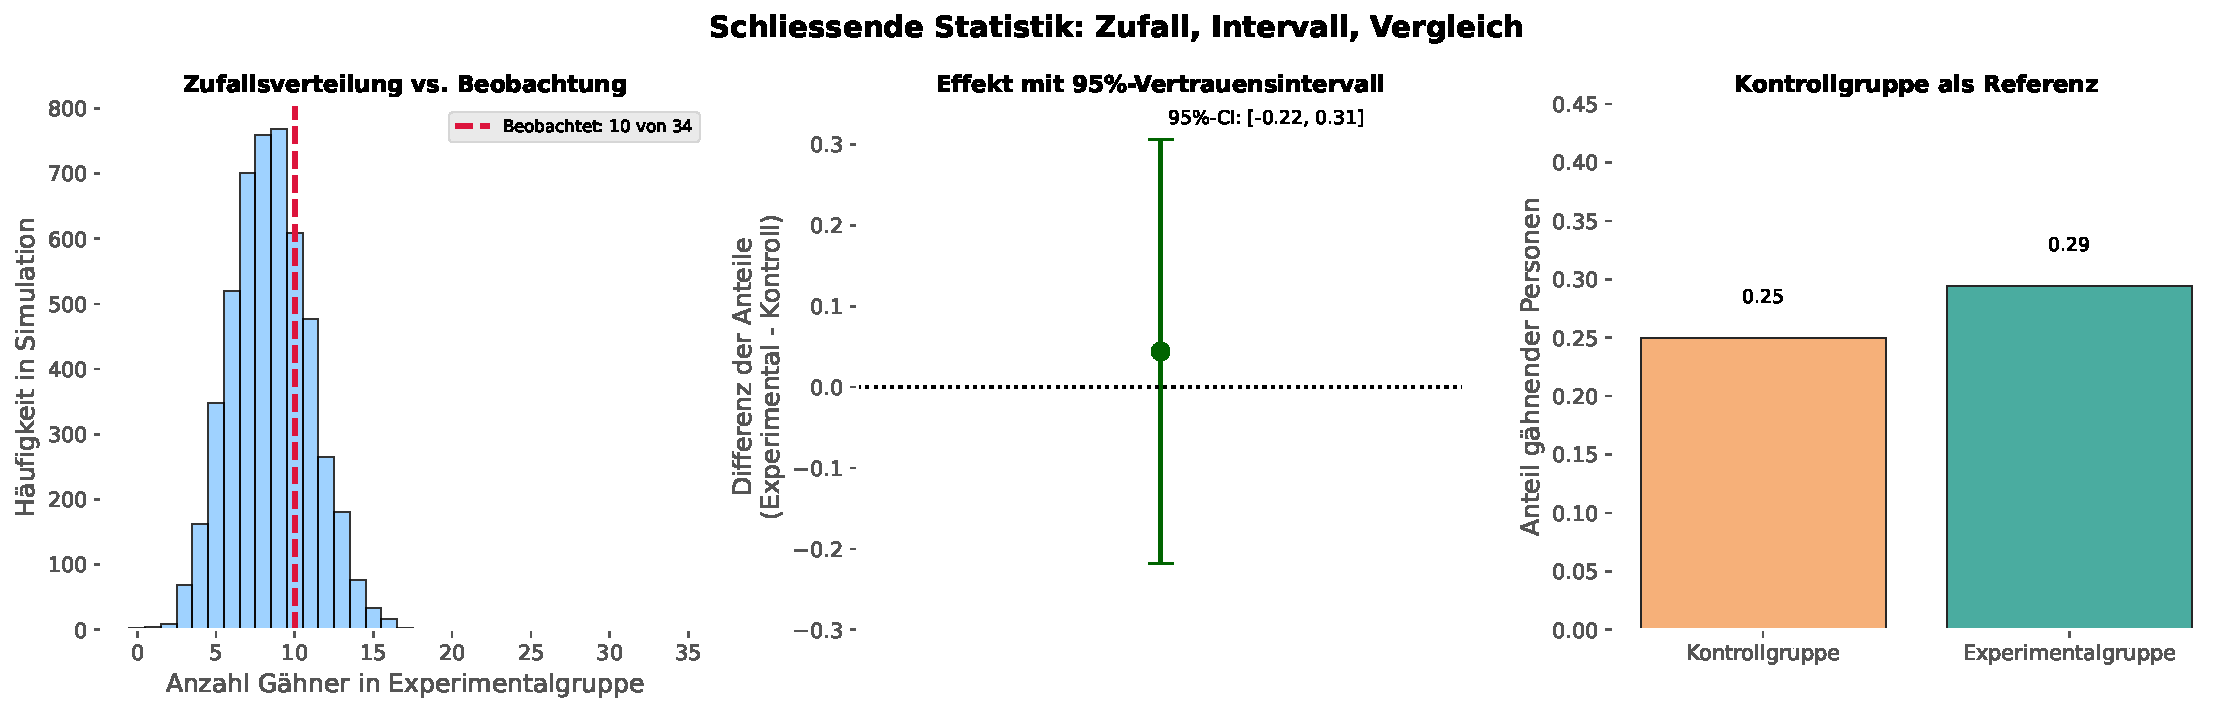
\includegraphics[width=0.95\textwidth]{Various/Wahlpflichtmodul Statistik/Figures/plots_inferential_basics.pdf}
    \end{figure}
\end{myexample}

\begin{myremark}
	Faustregel für dieses Modul: Bei grösserer Stichprobe wird das Vertrauensintervall meist enger.
\end{myremark}

\begin{mydefinition}
	Eine \textbf{Kontrollgruppe} dient als Vergleichsgruppe ohne Behandlung bzw. ohne den untersuchten Einfluss.
	Sie hilft, Unterschiede nicht vorschnell kausal zu deuten.
\end{mydefinition}

\begin{myexample}
	Wenn untersucht wird, ob ein Lernritual die Konzentration verbessert, braucht es idealerweise
	eine Gruppe mit Ritual und eine vergleichbare Kontrollgruppe ohne Ritual.
\end{myexample}

\subsection{Beispiel ``MythBusters'': Ist Gähnen ansteckend?}

\begin{myexercise}
	Verwenden Sie das vollständig durchgerechnete Beispiel oben:
	\[
		\hat{\Delta}=4.4\text{ Prozentpunkte},
		\qquad
		95\%-Intervall\approx[-21.8\%,\,30.6\%].
	\]

	In einem zweiten, gleich aufgebauten Versuch werden in beiden Gruppen \textbf{mehr Personen} untersucht (grösseres $n$),
	wobei die beobachteten Anteile ähnlich bleiben.

	Bearbeiten Sie nur die folgenden Punkte:
	\begin{enumerate}
		\item Wird das Vertrauensintervall eher breiter oder eher schmaler? Begründen Sie in einem Satz.
		\item Was bedeutet diese Veränderung für die Präzision der Aussage?
		\item Bleibt die Rolle der Kontrollgruppe wichtig? Begründen Sie kurz.
	\end{enumerate}
	\begin{myanswer}
		Bei grösserem $n$ wird das Intervall in der Regel \textbf{schmaler}.

		Ein schmaleres Intervall bedeutet: Die Aussage ist präziser, die Unsicherheit kleiner.

		Ja, die Kontrollgruppe bleibt zentral, weil nur der Vergleich mit ihr zeigt, ob der beobachtete Unterschied über den Referenzzustand hinausgeht.
	\end{myanswer}
\end{myexercise}

\begin{mychallenge}
	\textbf{Optional vertieft: Formale Definition und Rechnung}

	Für den Vergleich zweier Gruppen betrachten wir die Differenz zweier Anteile
	\[
		\Delta = p_{\mathrm{exp}} - p_{\mathrm{kontr}}.
	\]
	Ein approximatives 95\%-Vertrauensintervall lautet
	\[
		\hat{\Delta} \pm 1.96 \cdot \mathrm{SE}(\hat{\Delta}),
		\qquad
		\mathrm{SE}(\hat{\Delta}) = \sqrt{\frac{\hat{p}_{\mathrm{exp}}(1-\hat{p}_{\mathrm{exp}})}{n_{\mathrm{exp}}} + \frac{\hat{p}_{\mathrm{kontr}}(1-\hat{p}_{\mathrm{kontr}})}{n_{\mathrm{kontr}}}}.
	\]

	Rechnen Sie das Gähn-Beispiel mit unveränderten Anteilen $\hat{p}_{\mathrm{exp}}\approx29.4\%$ und $\hat{p}_{\mathrm{kontr}}=25.0\%$ einmal für $n_{\mathrm{exp}}=20$, $n_{\mathrm{kontr}}=20$ und einmal für $n_{\mathrm{exp}}=80$, $n_{\mathrm{kontr}}=80$.
	Vergleichen Sie die Intervallbreiten und interpretieren Sie die Rolle von 0.
	\begin{myanswer}
		Die Breite des Vertrauensintervalls hängt mit der Stichprobengrösse zusammen: kleineres $n$ $\Rightarrow$ breiteres Intervall,
		grösseres $n$ $\Rightarrow$ schmaleres Intervall.

		Mit $\hat{\Delta}=4.4$ Prozentpunkten gilt:
		\begin{itemize}
			\item Für $n=20$: $\hat{p}_{\mathrm{exp}}\approx29.4\%$, $\hat{p}_{\mathrm{kontr}}=25.0\%$, $\hat{\Delta}=4.4$ Prozentpunkte.
			      $\mathrm{SE}(\hat{\Delta})=\sqrt{0.294\cdot0.706/20+0.25\cdot0.75/20}\approx0.141$.
			      95\%-Intervall: $0.044 \pm 1.96 \cdot 0.141 = [ -0.231, 0.320 ]\approx[-23.1\%,\,32.0\%]$ (enthält 0).

			\item Für $n=80$: $\hat{p}_{\mathrm{exp}}\approx29.4\%$, $\hat{p}_{\mathrm{kontr}}=25.0\%$, $\hat{\Delta}=4.4$ Prozentpunkte.
			      $\mathrm{SE}(\hat{\Delta})=\sqrt{0.294\cdot0.706/80+0.25\cdot0.75/80}\approx0.070$.
			      95\%-Intervall: $0.044 \pm 1.96 \cdot 0.070 = [ -0.094, 0.182 ]\approx[-9.4\%,\,18.2\%]$ (enger, enthält 0 aber weiterhin).
		\end{itemize}
	\end{myanswer}
\end{mychallenge}

\section{Eigene Fragestellungen der SuS und Transfer}

\begin{myremark}
	Zur Findung statistisch aussagekräftiger Fragestellungen hat sich ein Ablauf in vier Schritten bewährt:
	\begin{itemize}
		\item \textbf{1. Gute Fragestellung klären}: Variabilität, Zielgruppe, Vergleich.
		\item \textbf{2. Daten beschreiben}: Skalenniveau, passende Kennzahlen und Diagramme.
		\item \textbf{3. Schliessend prüfen}: Unterschiede/Zusammenhänge mit Unsicherheit beurteilen.
		\item \textbf{4. Rückbezug auf eigene Frage}: Aussagebereich, Grenzen, nächste Schritte.
	\end{itemize}
\end{myremark}

\begin{myexercise}
	Formulieren Sie eine eigene statistische Fragestellung aus Ihrem Interesse (z.B. Schlaf, Mediennutzung, Sport, Lernen).
	Grenzen Sie Zielgruppe und Aussagebereich explizit ein und notieren Sie, welche Daten Sie dafür benötigen.

	\begin{myanswer}
		Eine gute Antwort nennt eine variable Grösse, eine konkrete Zielgruppe und mindestens einen sinnvollen Vergleich.
		Zusätzlich wird klar benannt, welche Aussage mit den geplanten Daten möglich ist und was offen bleibt.
	\end{myanswer}
\end{myexercise}

\section{Mini-Checkliste: Statistik in Texten und Grafiken}

\begin{myexercise}\label{myexercise:checkliste}
	Finden Sie einen Online-Artikel, der eine Statistik-Grafik enthält. Überprüfen Sie die Grafik kritisch anhand der folgenden Checkliste:
	\begin{itemize}
		\item[$\square$] Woher stammen die Daten (Quelle)?
		\item[$\square$] Wie gross ist die Stichprobe?
		\item[$\square$] Wird Median oder Mittelwert verwendet und passt das?
		\item[$\square$] Startet die Achse bei 0?
		\item[$\square$] Werden Prozente mit absoluten Zahlen verwechselt?
		\item[$\square$] Fehlen wichtige Gruppen oder Werte?
		\item[$\square$] Ist die Aussage in der Grafik mit der Datenlage vereinbar?
	\end{itemize}
\end{myexercise}
